\section{Motivation}
Our world is highly interconnected, with global supply chains working around the clock to ensure the flow of goods and services across the globe. Shipping, one of the oldest industries in the world, has played a crucial role in human evolution and economic development in all countries. With 75\% of the Earth consisting of water bodies, there are over 2500 ports worldwide that handle more than 50,000 professional merchant vessels and hundreds of thousands of smaller vessels, and the shipping industry provides direct and indirect employment to more than 2 million people worldwide. \cite{donepudi2014technology}. Like every industry, the shipping industry is also undergoing various technological revolutions in the age of the fourth industrial revolution, such as autonomous vessels, smarter supply chains, logistics, etc. These innovations are partially influenced by research and rapid adoption in other automotive and logistic industries.
\begin{figure}[H]
    \centering
    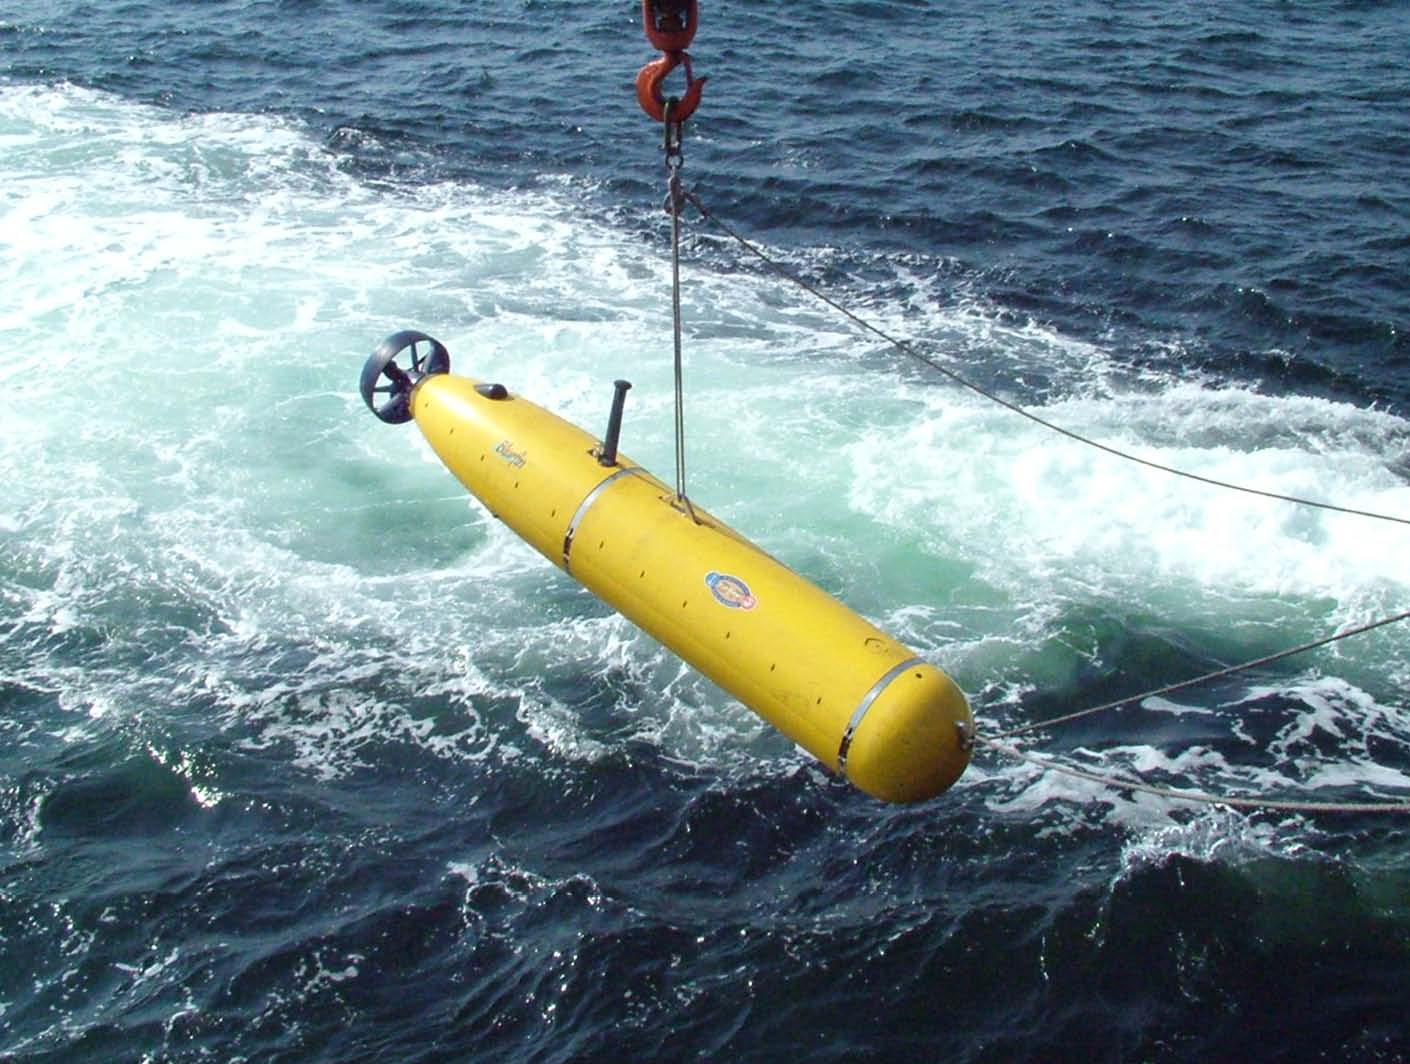
\includegraphics[width=\textwidth,height=6cm,keepaspectratio=true]{src/Images/BPAUV-MP_from_HSV-.jpg}
    \caption{Battlespace Preparation Autonomous Underwater Vehicle (BPAUV) from Bluefin Robotics}\cite{auv_img}
\end{figure}
\\

Autonomous maritime technology was first commercially applied to the maritime industry in the late 1990s as Autonomous Underwater Vehicles (AUV). These were primarily used for inspection and exploration purposes. With oil and gas companies moving toward deeper waters, there was a need for cheaper and more reliable pipeline inspection and operations. Since then, autonomous technologies for various applications have been developed for smoother operations of global fleets. These applications include hull inspection, port surveillance, and, recently, autonomous vessels. \cite{ghaderi2019autonomous}
\begin{figure}[H]
    \centering
    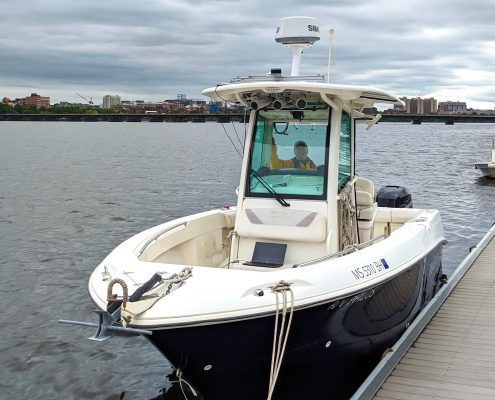
\includegraphics[width=\textwidth,height=7cm,keepaspectratio=true]{src/Images/robo_whaler.jpg}
    \caption{
     R/V Philos (RoboWhaler\cite{defilippo2021robowhaler}) is a recreational marine vessel capable of level 1 - level 5 autonomous operations developed by MIT's Sea Grant laboratory}
\end{figure}
\\

Autonomous Surface Vehicles, or ASVs, were first developed at the academic level in 1993 when MIT presented its first vessel, called ARTEMIS. The goal of this ship was to collect bathysphere data along the Charles River in Cambridge, Massachusetts. Since then, many more institutes have started researching the field of autonomy on board increasingly larger vessels. The most recent proposal by Rolls-Royce and Man Diesel aims to automate bulk and cargo shipping vessels\cite{schiaretti2017survey}. Our work was mainly inspired by the work of Michael DeFilippo et al.\cite{defilippo2021robowhaler}. The Sea Grant team actively collects data and conducts marine autonomy experiments along the Charles River in Cambridge, Massachusetts, and were a great source of inspiration, learning, data, and testing. Our work hopes to build upon VAIS\cite{Zhang_2015_CVPR_Workshops} work of using COLREGs compliant perception ontology by defining a leaner base ontology for researchers to work from and review current state-of-the-art computer vision models in order to be more applicable in any future COLREG-based ASV development. There are many other maritime datasets developed and published as surveyed by \cite{su2023survey}. Some notable examples include MARVEL\cite{gundogdu2017marvel}, LaRS\cite{Zust_2023_ICCV}. Other similar work includes developing obstacle avoidance systems based on COLREGS such as \cite{zhao2019colregs}\cite{kuwata2013safe}\cite{naeem2012colregs} but does not define a perception ontology.

